%% Theoretischen_Bezug.tex
%% $Id: Theoretischen_Bezug.tex 61 2012-05-03 13:58:03Z bless $
%%

\chapter{Theoretischen Bezug und bisheriger Forschungsstand }
\label{ch:Theoretischen_Bezug}


Zum derzeitigen Zeitpunkt gibt es unterschiedliche Ansätze der Forschung im Controlling, speziell in der Konzeption. In den letzten 20 Jahren hat sich zudem die Ausrichtung weg von einer rein wirtschaftlichen Teildisziplin bis hin zur eigenständigen Controlling Funktion entwickelt.
\\
Wie bereits in Punkt eins erwähnt stellt sich die Frage nach dem Unterschied im Controlling zwischen Theorie, Konzeption und Praxis. Wie in Abbildung \ref{fig:Controllingkonzeption} zu sehen ist, gibt es nach Scherm und Pietsch gibt es eine große Anzahl an Konzeptionen die zwischen klassischen und neuen Konzeptionen des Controllings unterschieden werden.

\begin{figure}[H]
 \centering
 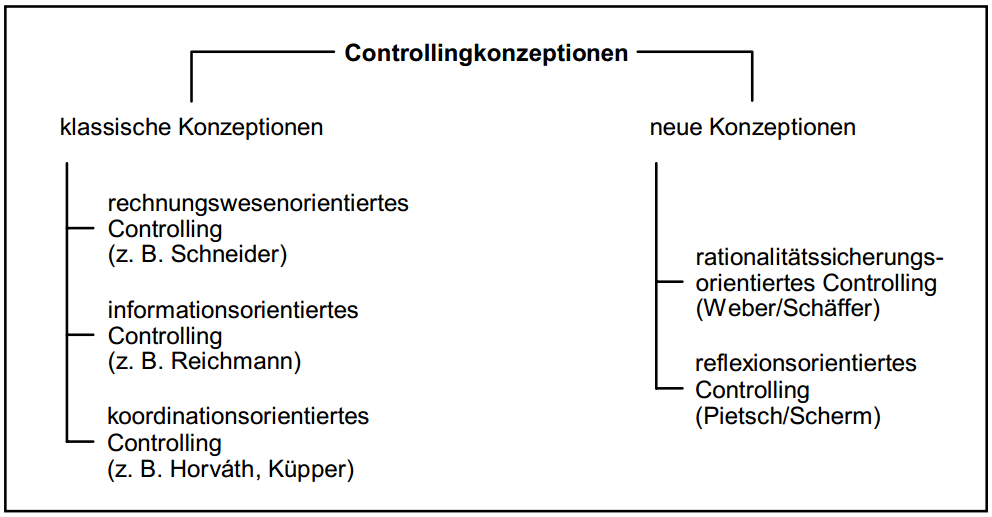
\includegraphics[scale=0.45]{images/Controllingkonzeption.png}
 \caption{Controllingkonzeptionen \cite{fig:Controllingkonzeption}}
 \label{fig:Controllingkonzeption}
\end{figure}

Während sich die klassischen Konzeptionen auf Rechnungswesen orientiertes, informationsorientiertes und koordinationsorientiertes Controlling die klassischen Konzeptionen wiederspiegeln, handelt es bei den neuen Konzeptionen um jene, die sich mit Entscheidungen und Sicherstellung der Führungsrationalität befasst.
\\
Diese Konzeptionen können mit den Kundenorientierten Controlling Ansätzen innerhalb der T-Systems verglichen werden.


%%% Local Variables: 
%%% mode: latex
%%% TeX-master: "thesis"
%%% End: 
